\documentclass[conference]{IEEEtran}
\IEEEoverridecommandlockouts
% The preceding line is only needed to identify funding in the first footnote. If that is unneeded, please comment it out.
\usepackage{cite}
\usepackage{amsmath,amssymb,amsfonts}
\usepackage{algorithmic}
\usepackage{graphicx}
\usepackage{textcomp}
\usepackage{xcolor}
\usepackage{hyperref}
%% ODE handling
\usepackage{diffcoeff}
\usepackage{booktabs}
%% The SI units alignment
\usepackage{siunitx}
\def\BibTeX{{\rm B\kern-.05em{\sc i\kern-.025em b}\kern-.08em
    T\kern-.1667em\lower.7ex\hbox{E}\kern-.125emX}}

% upright sub-index
\newcommand{\ui}[2]{#1 _{\text{#2}}}
% upright sub-index with variable
\newcommand{\uis}[3]{#1 _{\text{#2}, #3}}

\begin{document}

\title{DNN-based Dictionary-Free Method for Identifying Linear Model of Nonlinear System with Input Delay\\
    \thanks{Identify applicable funding agency here. If none, delete this.}
}

\author{\IEEEauthorblockN{1\textsuperscript{st} Patrik Valábek}
    \IEEEauthorblockA{\textit{Department of Information Engineering and Process Control} \\
        \textit{Slovak University of Technology in Bratislava}\\
        patrik.valabek@stuba.sk}
    \and
    \IEEEauthorblockN{2\textsuperscript{nd} Marek Wadinger}
    \IEEEauthorblockA{\textit{Department of Information Engineering and Process Control} \\
        \textit{Slovak University of Technology in Bratislava}\\
        0000--0002--0167--6331}
    \and
    \IEEEauthorblockN{3\textsuperscript{rd} Martin Klaučo}
    \IEEEauthorblockA{\textit{Department of Information Engineering and Process Control} \\
        \textit{Slovak University of Technology in Bratislava}\\
        0000--0003--0098--2625}
}

\maketitle

\begin{abstract}
    Nonlinear dynamical systems with input delays pose significant challenges for prediction, estimation, and control due to their inherent complexity and the impact of delays on system behavior. Traditional linear control techniques often fail in these contexts, necessitating innovative approaches. This paper presents a dictionary-free method for learning linear representations of nonlinear systems with input delays using deep neural networks (DNNs). Leveraging the Koopman operator framework, which globally linearizes nonlinear dynamics, we address the limitations of extended Dynamic Mode Decomposition (eDMD). While eDMD enhances model capability with nonlinear measurements, its reliance on predefined dictionaries constrains its accuracy. Our approach uses DNNs to automatically generate and update nonlinear transformations, enabling the learning of high-fidelity Koopman operator models. Additionally, we incorporate time-delayed embeddings to account for input delays, ensuring precise modeling and improved long-term forecasting of nonlinear dynamics. Our method provides a robust framework for modeling nonlinear systems with input delays, offering significant advancements over existing techniques.
\end{abstract}

\begin{IEEEkeywords}
    DNN, Koopman analysis, LSTM, nonlinear systems, input delays
\end{IEEEkeywords}

\section{Introduction}
Understanding and controlling nonlinear dynamical systems is a fundamental challenge across various scientific and engineering disciplines. Traditional linear control techniques often fall short when applied to such systems due to their inherent nonlinearity. A promising approach to this problem is the identification of coordinate transformations that render nonlinear dynamics approximately linear, thus enabling the application of linear theory for prediction, estimation, and control.

Koopman analysis, a technique that facilitates the linearization of nonlinear systems through the Koopman operator, has gained considerable traction in recent years~\cite{Mezic2004101, Mezić2005}. The Koopman operator offers a global linearization of dynamics by mapping the original nonlinear system into a higher-dimensional space where the dynamics can be represented linearly. This method is particularly appealing because it shifts the complexity from the system's equations to the eigenfunctions of the Koopman operator, which span an invariant subspace and allow the dynamics to be described by a matrix within this subspace.

Finite-dimensional approximations of the Koopman operator are often achieved using Dynamic Mode Decomposition (DMD), introduced by Schmid. While DMD identifies spatio-temporal coherent structures from high-dimensional systems, it typically fails to capture nonlinear transients due to its reliance on linear measurements. To address this, Extended DMD (eDMD) incorporates nonlinear measurements, improving its capability to model nonlinear systems. However, eDMD faces challenges such as high dimensionality and closure issues, which arise because there is no guarantee that the nonlinear measurements form a Koopman invariant subspace~\cite{Lusch2018}. Consequently, the identification and representation of Koopman eigenfunctions remain crucial tasks, motivating the use of advanced deep learning techniques.

To overcome the limitations of eDMD, deep neural networks (DNNs) have been employed to learn Koopman operator representations. DNNs remove the bottleneck of predefined dictionaries by creating linear representations of a system through nonlinear transformations of individual neurons. These neurons combine to form complex functions parametrized by tunable weights and biases, allowing the network to adaptively learn the optimal transformations during training. This approach significantly enhances the fidelity of Koopman operator models, particularly in multi-step prediction tasks, thus improving long-term forecasting of nonlinear dynamics~\cite{Yeung2019}.

An important aspect of modeling dynamical systems is accounting for time-delays, which are common in many physical and industrial processes. Time-delay can significantly affect system behavior and control performance. Introducing time-delayed embeddings of control action in DMD improves identification of system with input delays, while does not explicitly identify the time-delays. Various methods exist to identify and model time-delays, including state-space realization approaches and correlation analysis. The state-space realization approach involves constructing a state-space representation based on input-output data from experiments, extracting time-delay information from the system's impulse response~\cite{Lima2015254}. Correlation analysis, on the other hand, focuses on identifying time-delays in dynamic processes with disturbances, aiming to improve control accuracy and stability~\cite{Li201792}.

This paper presents a dictionary-free method for learning linear representations of nonlinear systems with input delays using deep neural networks. By leveraging the strengths of deep learning in generating and updating nonlinear transformations, our approach aims to overcome the limitations of traditional Koopman operator methods and provide a robust framework for modeling and controlling nonlinear systems with time-delays. The following sections will delve into the theoretical background, methodological innovations, and practical applications of our approach, guiding the reader through the key challenges and solutions in this domain.

\section{Methodology}

\section{Results}

\subsection{Comparison with eDMD}

Here we compare the performance of DeReK with eDMD on a simulated two tank system without interaction with an input delays. The system is described by the following equations:

\begin{equation}\label{eq:two_tanks_system}
    \begin{aligned}
        \diff{h_1(t)}{t} & = q(t-\tau) - \frac{k_1}{F_1}\sqrt{h_1(t)}                     \\
        \diff{h_2(t)}{t} & = \frac{k_1}{F_2}\sqrt{h_1(t)} - \frac{k_2}{F_2}\sqrt{h_2(t)},
    \end{aligned}
\end{equation}

where \(h_1(t)\) and \(h_2(t)\) are the water levels in tanks 1 and 2, respectively, \(q(t)\) is the input flow rate, \(\tau \) is the input delay, and \(k_1\), \(k_2\) are the flow rate constants of the valves and \(F_1\), \(F_2\) are the cross-sectional areas of the tanks.

The experimental data were acquired by simulating this system at sampling period \( \ui{T}{s} = 10 \, \mathrm{s} \) with input delay \( \tau = 2\ui{T}{s} \). Random change in the input flow rate from the interval \( \ui{q}{min} = 0.0 \, \text{m}^3\text{s}^{-1} \), \( \ui{q}{max} = 0.03 \) \( \text{m}^3\text{s}^{-1} \) was applied to the system.

The data were split into training and testing sets with a ratio of 50:50. The training set was used to train the models, while the testing set was used to evaluate their performance. The models were trained to predict the water levels in tanks 1 and 2 for the whole testing set based on the applied input flow rate and the initial state of the system.

eDMD used dictionary of polynomials up to degree 2, square root and inversion of the water levels, and time-delayed embeddings of the input flow rate composed of previous 20 samples. Lifted states were obtained by concatenating the dictionary terms and time-delayed embeddings, and the Koopman matrix was learned using eDMD.

The DeReK model consists of an LSTM layer with one hidden layer with 8 units, to extracts information about the time delays in the system from the history of the system. The concatenated information is then transformed to lifted states using an encoder layer with a fully connected network. The lifted states are further concatenated with the input flow rate using another concatenation layer.

Figure~\ref{fig:two_tanks_results} shows the predicted and actual water levels in tanks 1 and 2 for the two tank system using eDMD and DeReK. The results demonstrate that DeReK outperforms eDMD in terms of prediction accuracy, capturing the system's dynamics more effectively over the testing set. eDMD exhibits systematic positive bias in the prediction of water levels, while DeReK provides more accurate and consistent predictions. Nevertheless, the linear model generated by DeReK displays non-minimum phase behavior, which is a common issue in identification of systems with input delays.

\begin{figure}[htbp]\label{fig:two_tanks_results}
    \centerline{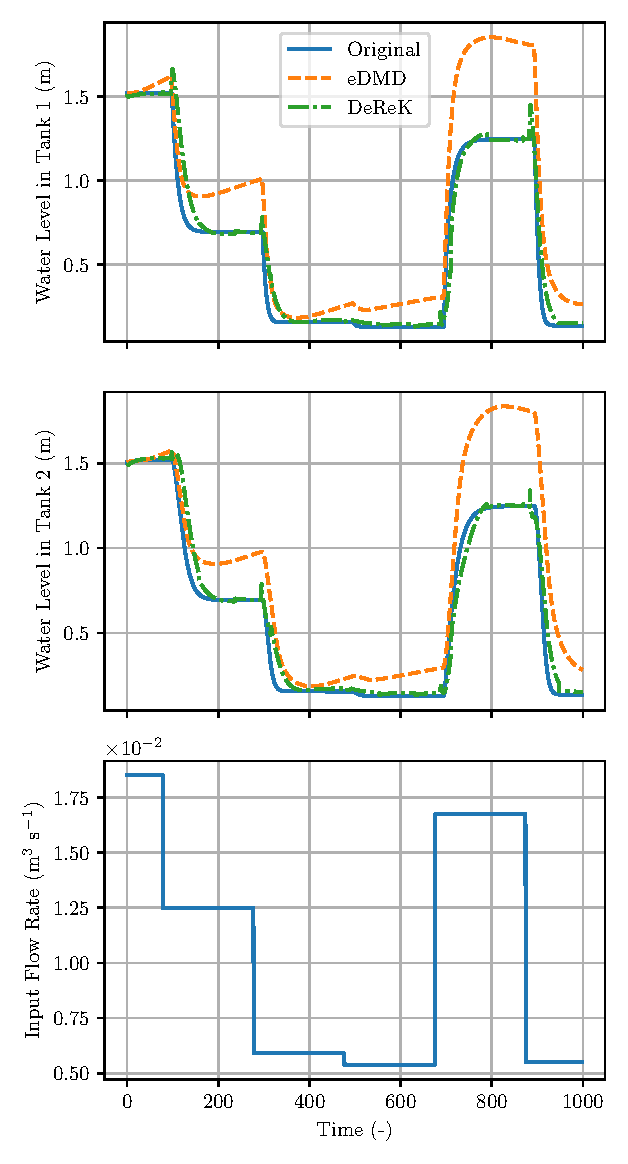
\includegraphics[width=\linewidth]{figures/dmdc_multipred-r0-hn20-polydeg2-inv1.pdf}}
    \caption{Predicted and actual water levels in tanks 1 and 2 for the two tank system}
\end{figure}

The performance of the models was evaluated using the mean absolute error (MAE) and the sum of the absolute differences (SAD) between the predicted and actual water levels in tanks 1 and 2. The results are presented in Table~\ref{tab:two_tanks_results}. DeReK achieved a significantly lower MAE and SAD compared to eDMD, indicating its superior performance in modeling the two tank system with input delays.

\begin{table}[htbp]\label{tab:two_tanks_results}
    \caption{Performance comparison of DeReK and eDMD on the two tank system with input delays}
    \begin{center}
        \begin{tabular}{c| S[table-format=1.4] S[table-format=3.2]}
            \toprule
            \textbf{Model} & \textbf{MAE} & \textbf{SAD} \\
            \midrule
            eDMD           & 0.5200       & 92.23        \\
            DeReK          & 0.0922       & 520.03       \\
            \bottomrule
        \end{tabular}
    \end{center}
\end{table}



\bibliographystyle{IEEEtran}
\bibliography{main}

\end{document}
